\documentclass[cheatsheet.tex]{subfiles}
\begin{document}
\subsection{Decision Tree}
A \textbf{decision tree} partitions the instance space by branching on feature values (literals), with leaves representing the learned concept. \textbullet Each leaf represents a conjunction of literals on its path \textbullet The learned concept is the disjunction of the positive leaves: $L_1 \vee{L_2} \vee{L_3}$. \textbullet maximally expressive. they
can separate any consistently labeled data -- Thus more powerful than the conjunctive hypothesis space, overfitting.
\textbullet \textbf{Simplify decision tree}: Merge feature labels and test the difference, Enforce a depth limit, Enforce a purity threshold, Enforce a purity increment threshold, Build the complete tree and then iteratively merge leaves based on lowest purity decrease up to a number of leaves $N$ or a purity $\delta$, Combinations of depth and purity measures.
\subsection{Ranking \& Probabilities}
\textbullet Use empirical probabilities(Using Laplace correction) $\dot{p}$ - for segments $i$ and $j$, order $i>j$ if $\dot{p}_i>\dot{p}_j$ \textbullet Ranking is with respect to a particular class (e.g., dolphin) \textbullet A ranking is on a set of m instances  $X = \{ x_1, ..., x_m \}$ \textbullet A decision tree with N leaves will have N different ranks \textbullet We can use those empirical probabilities (for each class) calculated for every leaf to create a probability estimation tree(Using Laplace correction)\\
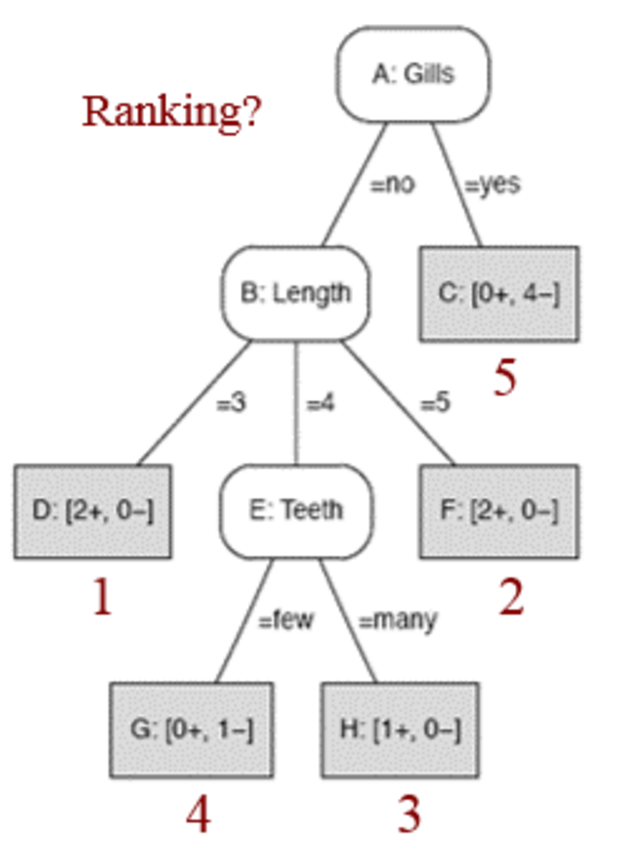
\includegraphics[width=40mm]{ranking_tree.png} 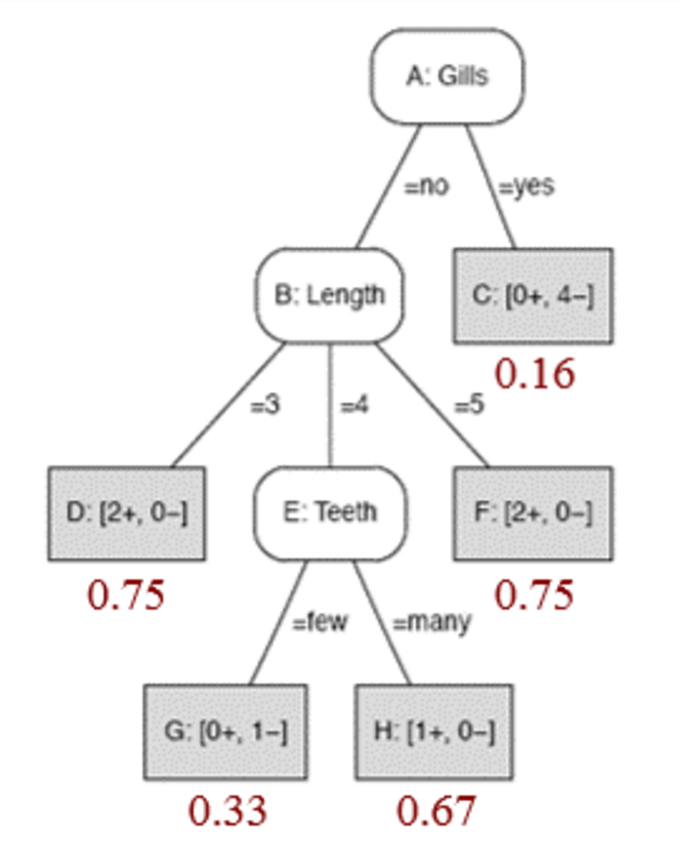
\includegraphics[width=40mm]{probability_tree.png}
\subsection{Tree learning as Variance reduction}
skipped
\end{document}
